\documentclass{article}
\usepackage{color,soul}
\usepackage{amsmath}
\usepackage{amsfonts} 
\usepackage{eqnarray}
\usepackage{bm}
\usepackage{multirow}
\usepackage{graphicx}
\usepackage{booktabs}
\usepackage{comment}
\usepackage{subcaption}
\usepackage{listings}
\usepackage[margin=0.5in]{geometry}

\title{School of Electrical and Computer Engineering\\
Purdue University, WL, IN, USA}
\author{Nahian Ibn Hasan\\
Email: hasan34@purdue.edu\\
PUID: 0032764564\\
ECE66100 - Computer Vission\\
Fall 2022\\
Homework-7}
\date{\today}

\begin{document}
\maketitle
\section{Objective}
In this homework, we will explore different ways of representing the textures in images such as Local Binary pattern (LBP), Gram Matrix (GM), Adaptive Instance Normalization (AdaIN) etc.
\section{Theoretical Questions}
\subsection{Question 1}
The reading material for Lecture 16 presents three different approaches to characterizing the texture in an image: 1) using the Gray Lcale Co-Occurrence Matrix (GLCM); 2) with Local Binary Pattern (LBP) histograms; and 3) using a Gabor Filter Family. Explain succinctly the core ideas in each of these three methods for measuring texture in images. (You are not expected to write more than a dozen sentences on each).
\subsection*{Answer}
\par \textbf{GLCM}: The basic idea of the GLCM matrix is to estimate the joint probability distribution $P[x_1,x_2]$ for the gray scale values of an image when the pixels $(x_1,x_2)$ are at a specific distance $d$ from each other. The shape of this joint probability distribution is used to characterize the texture of an image. If there ae $M$ gray-scale levels in an image, the shape of the GLCM matrix will be $M\times M$. If the order of the pixels $(x_1,x_2)$ doesn't matter, then the GLCM matrix will be a symmetric matrix, otherwise it would be an asymmetric one. Dividing each element of the GLCM matrix by the total number of occurences will provide the joint probability distribution for every gray-level. There are different characterization metrics for GLCM matrices. Perhaps, the most popular one is tthe Entropy. If the GLCM matrix is of size $M\times M$, the highest entropy achievable for a GLCM matrix is $M$, when the probability distribution is uniform (i.e. all the elements of the GLCM are complete random). On the other hand, the worst possible entropy is $0$ when all the pixels have the same gray-scale. Apart from it, there are other metrics as well such as, Energy, Contrast, Homogeneity.
\par \textbf{LBP}: LBP is another way to characterize the rotationally and grayscale invariant texture of an image. The fundamental idea is to find out the local binary pattern of a pixel through runs of 0's and 1's. Let's say, we find out the $P$ neighboring points around a pixel, which are located on a circle of radius $R$ as follows-
\begin{equation}
	(\Delta u , \Delta v) = \bigg(Rcos\big(\frac{2\pi p}{P}\big),Rsin\big(\frac{2\pi p}{P}\big)\bigg); p=0,1,2,\cdots, P
\end{equation}
If the pixels on the circles are coincident with the neighboring pixel's center, then the gray-level corresponding to that circle point is equal to the gray level of the coincident pixel. Otherwise, a bilinear interpolation technique can be used to interpolate the gray level at the circle point. If the predicted gray level at the circle point is greater than or equal to the gray level at the center pixel (around which the circle is drawn), then the entry for this circle point is considered 1, otherwise 0. Hence, for each pixel, we will get a binary pattern of 1's and 0's of length P. Next, following the criteria of LBP cerators, we can encode a single number for each of these patterns. By counting the number of occurences of each of these individual encoded information, we can form a histogram across all pixels of the image. This LBP histogram characterizes the texture of the image.

\par \textbf{Gabor FIlter Family} : Gabor filters capture the image texture at different spatial location for a certain frequency and firection. LBP captures the macro-level features, whereas Gabor filters are suitable for capturing micro-patterns that compose a macro-level pattern. Each Gabor filter can be considered as a highly localized Fourier Transform where a Gaussian decay function captures the localization at each pixel. A popular implementation of MPEG-7 makes 30 measurements on a texture at 6 orientations and 5 spatial frequency bands. A bank of Gabor filters (oriented at different directions) are convolved with an image which captures the best possible response at edges. 
\subsection{Question 2}
With regard to representing color in images, answer Right or Wrong for the following questions and provide a brief justification for each (no more than two sentences):
\begin{itemize}
	\item[a.] RGB and HSI are just linear variants of each other.
	\item[b.] The color space L*a*b* is a nonlinear model of color perception.
	\item[c.] Measuring the true color of the surface of an object is made difficult by the spectral composition of the illumination.
\end{itemize}
\subsection*{Answer}
\begin{itemize}
	\item[a.] \textbf{Wrong}. Each element of HSL color space define the Hue (H), Saturation (S) and Lightness (L). The RGB space defines the intensity level three primary colors Red (R), Green (G) and Blue (B) .
	\item[b.] \textbf{Right}. L*a*b* has three axes and each of these axes are non-linear. It's impossible to generate alinear mapping of the two-dimensional chromaticity diagram.
	\item[c.] \textbf{Right}. Any reflected light from the surface of an object depends on the intensity of the illuminating light and its properties and the spectral composition varies riddiculously depending on this. therefore, the true color perception is almost impossible. All we can do is to model it for different illuminant source.
\end{itemize}

\section{Implementation Notes}
\begin{itemize}
\item The LBP algorithm is run for different local circular radius (R) and number of pixels (P).
\item before applying the LBP algorithm, we resized the image to $64\times 64$ to make it faster.
\item The Python \textbf{BitVector} module is used to generate and encode the LBP histograms.
\item For Gram matrix construction, each image has been resized to $256\times 256$ for the sake of VGG19 model.
\item The normalized Gram matrix (GM) consists of $512\times 512$ pixels. For this project, we have considered different lengths of GM feature vector and record the result (i.e. accuracy).
\item The AdaIN-based feature vector estimation provides a feature vector of length $512\times 2$. Since for each channel, we only calculated the mean and variance across every pixel. We also varied the length of this ffeature vector and recorded the accuracy as well.
\item The classification was performed using a multiclass support vector machine (SVM).
\item Training and Testing data were almost uniformly distributed to avoid the class-imbalance issue. Fig. \ref{fig:sample_data} shows sample images from 4 classes.
\item The GM matrices and AdaIN feature vectors are calculated from the last Maxpooling layer of a pretrained VGG19 model. The pretrained network and its weigths are attached in the source code files.
\end{itemize}
\begin{figure}[!htbp]
     \centering
     \captionsetup[subfigure]{labelformat=empty}
    \includegraphics[width=0.60\textwidth]{../My_Code/Results/sample_data.png}
    \caption{Sample images from training set}
    \label{fig:sample_data}
\end{figure}

\newpage
\section{Results}
\subsection{Individual LBP Feature Vectors}
\begin{figure}[!htbp]
     \centering
     \captionsetup[subfigure]{labelformat=empty}
    \subcaptionbox{}{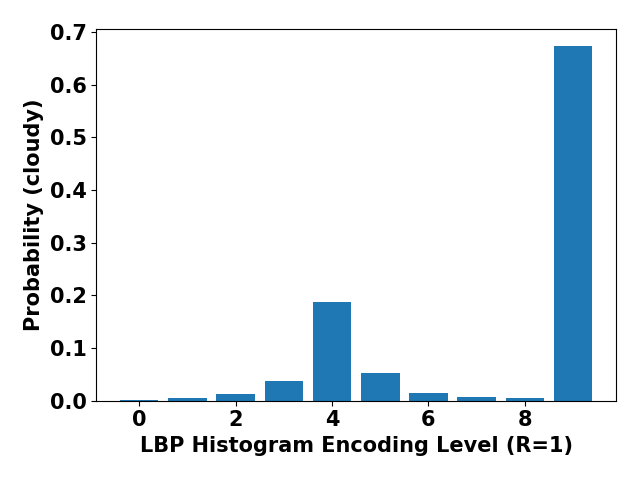
\includegraphics[width=0.245\textwidth]{../My_Code/Results/LBP_cloudy_R_1.png}}
    \subcaptionbox{}{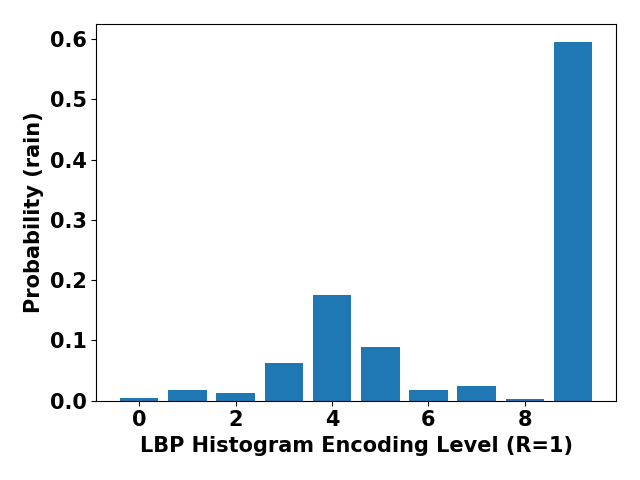
\includegraphics[width=0.245\textwidth]{../My_Code/Results/LBP_rain_R_1.png}}
    \subcaptionbox{}{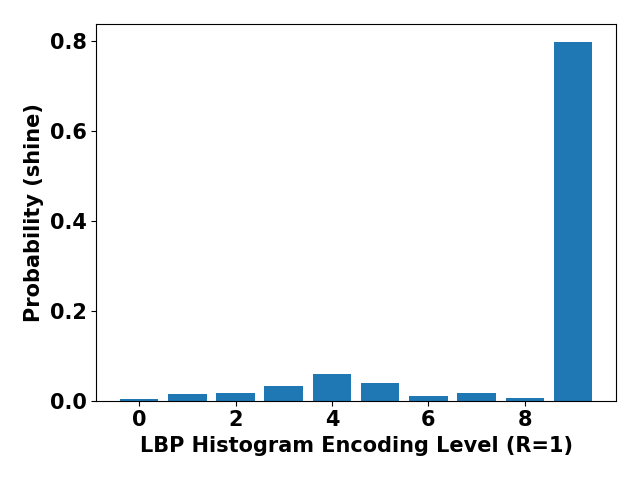
\includegraphics[width=0.245\textwidth]{../My_Code/Results/LBP_shine_R_1.png}}
    \subcaptionbox{}{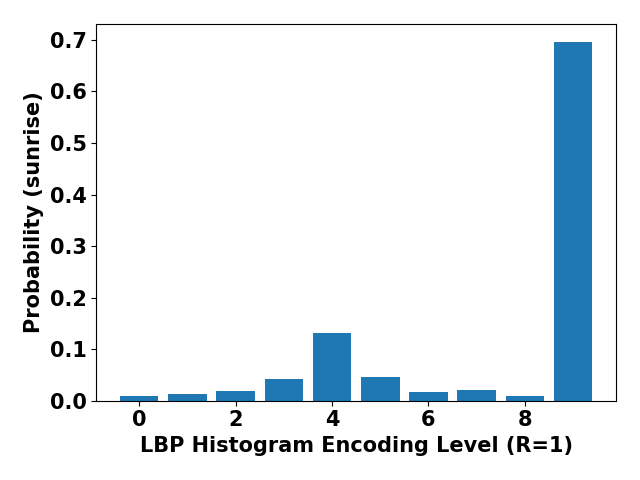
\includegraphics[width=0.245\textwidth]{../My_Code/Results/LBP_sunrise_R_1.png}}
    \subcaptionbox{}{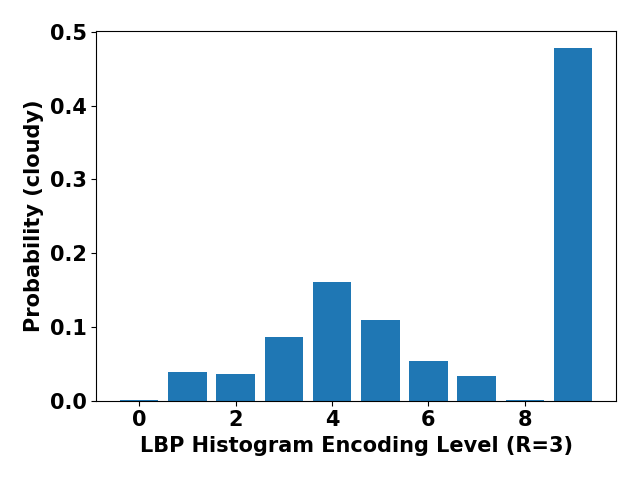
\includegraphics[width=0.245\textwidth]{../My_Code/Results/LBP_cloudy_R_3.png}}
    \subcaptionbox{}{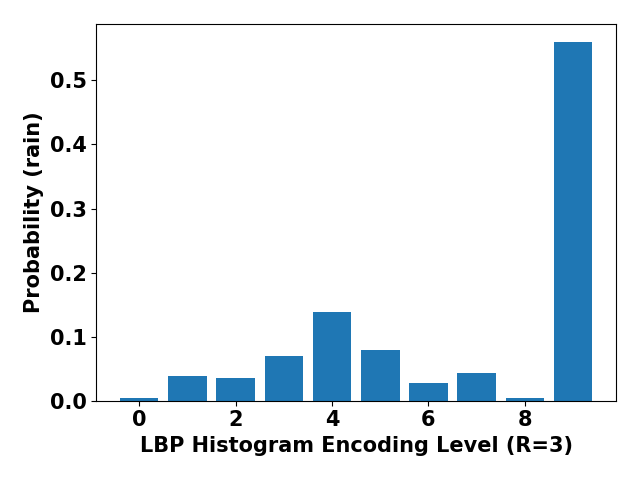
\includegraphics[width=0.245\textwidth]{../My_Code/Results/LBP_rain_R_3.png}}
    \subcaptionbox{}{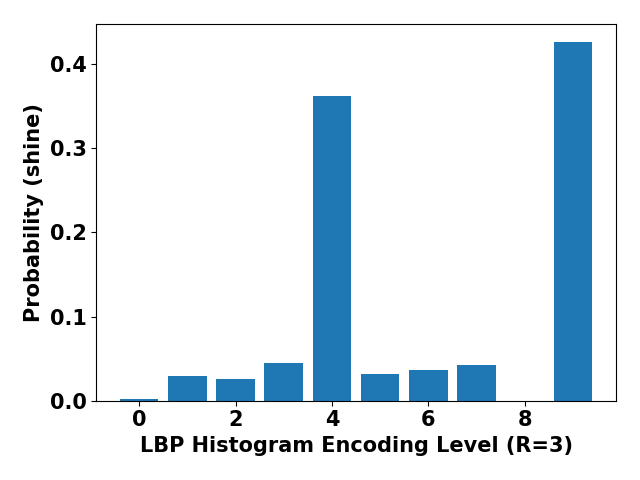
\includegraphics[width=0.245\textwidth]{../My_Code/Results/LBP_shine_R_3.png}}
    \subcaptionbox{}{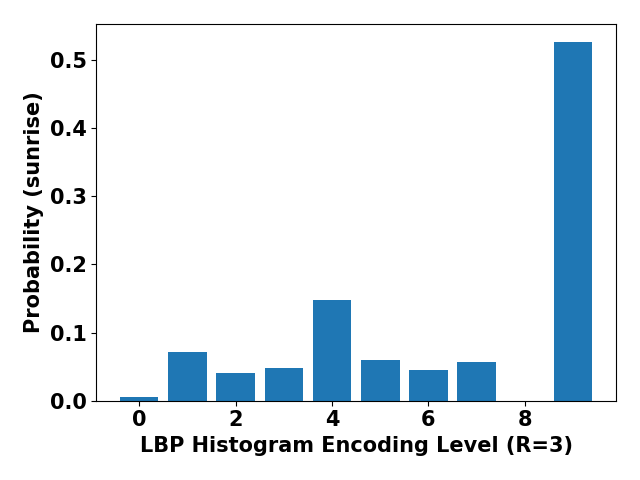
\includegraphics[width=0.245\textwidth]{../My_Code/Results/LBP_sunrise_R_3.png}}
    \subcaptionbox{}{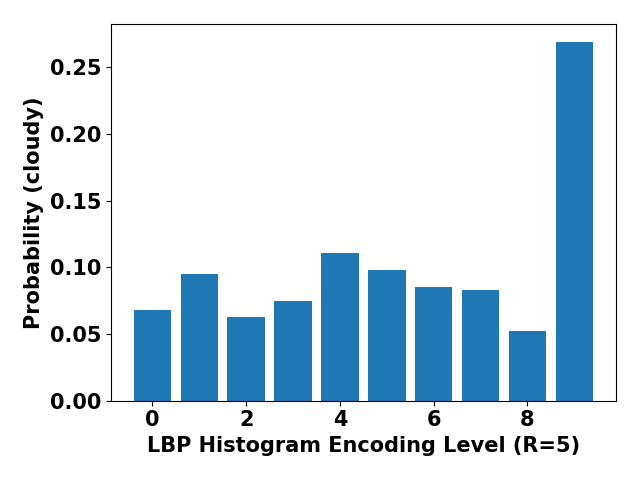
\includegraphics[width=0.245\textwidth]{../My_Code/Results/LBP_cloudy_R_5.png}}
    \subcaptionbox{}{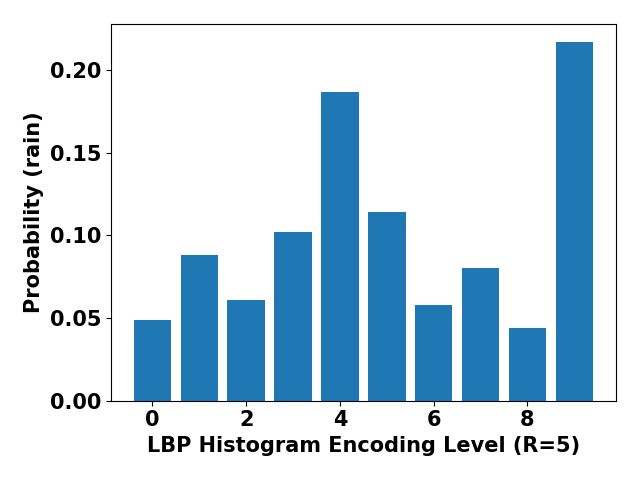
\includegraphics[width=0.245\textwidth]{../My_Code/Results/LBP_rain_R_5.png}}
    \subcaptionbox{}{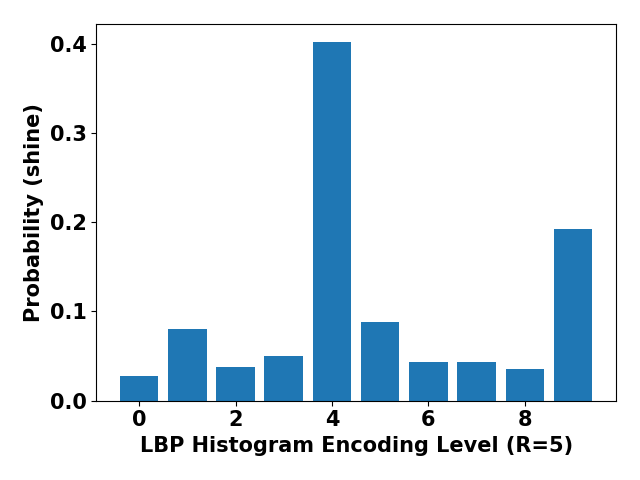
\includegraphics[width=0.245\textwidth]{../My_Code/Results/LBP_shine_R_5.png}}
    \subcaptionbox{}{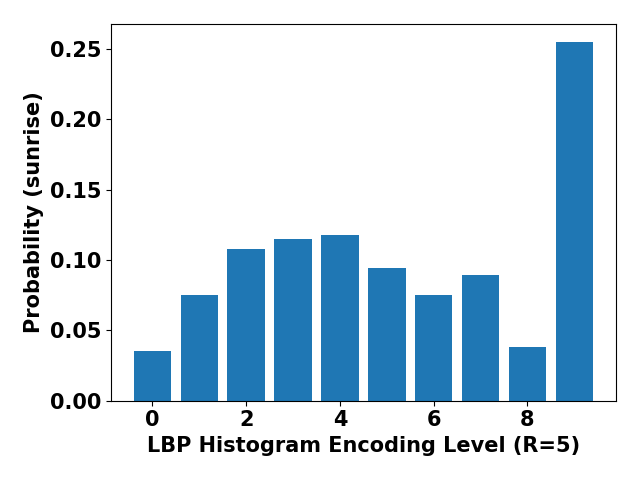
\includegraphics[width=0.245\textwidth]{../My_Code/Results/LBP_sunrise_R_5.png}}
    \subcaptionbox{}{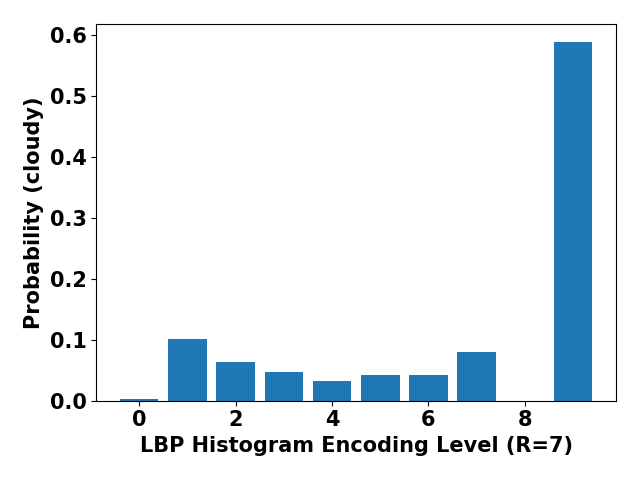
\includegraphics[width=0.245\textwidth]{../My_Code/Results/LBP_cloudy_R_7.png}}
    \subcaptionbox{}{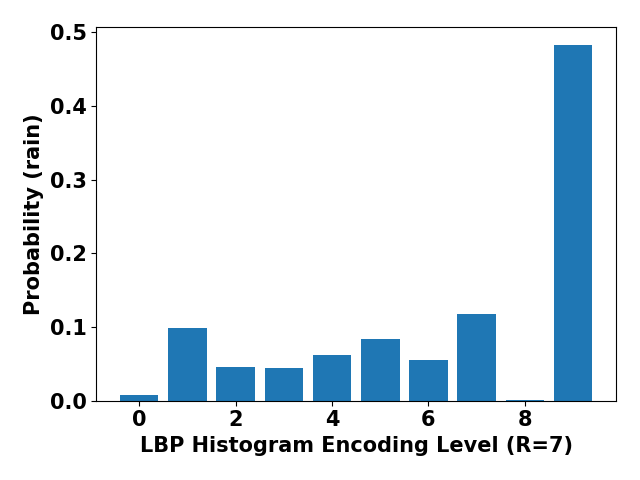
\includegraphics[width=0.245\textwidth]{../My_Code/Results/LBP_rain_R_7.png}}
    \subcaptionbox{}{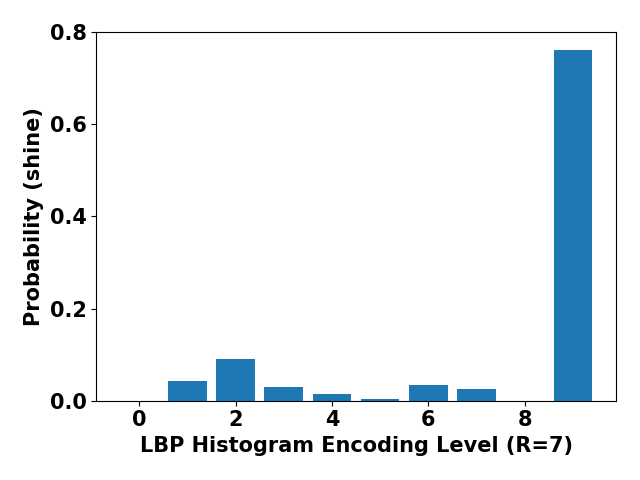
\includegraphics[width=0.245\textwidth]{../My_Code/Results/LBP_shine_R_7.png}}
    \subcaptionbox{}{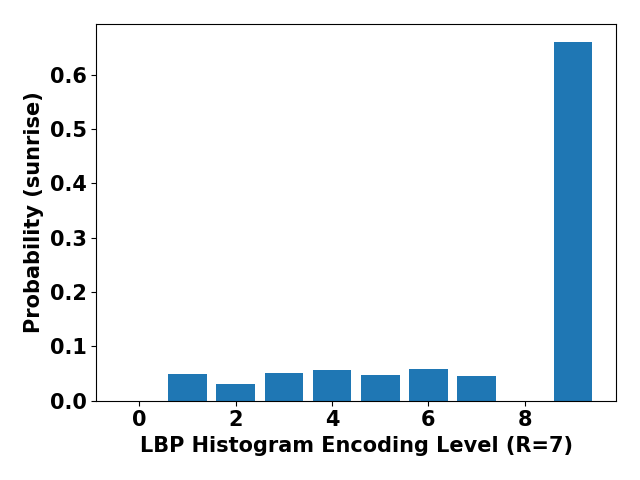
\includegraphics[width=0.245\textwidth]{../My_Code/Results/LBP_sunrise_R_7.png}}
    \subcaptionbox{}{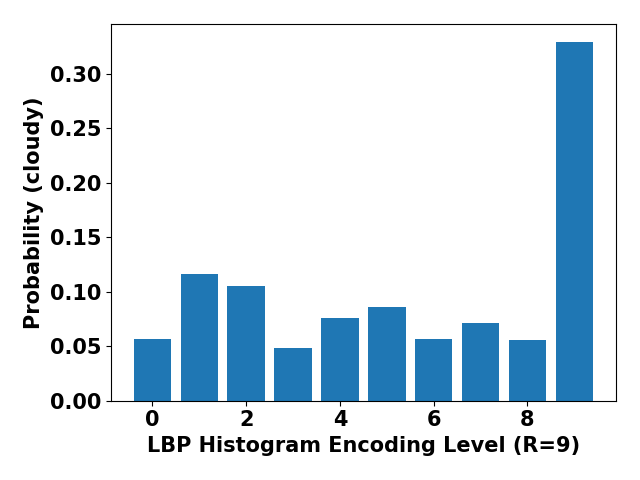
\includegraphics[width=0.245\textwidth]{../My_Code/Results/LBP_cloudy_R_9.png}}
    \subcaptionbox{}{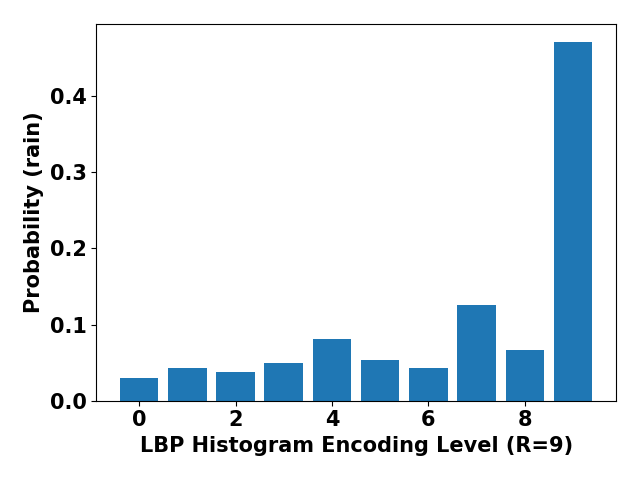
\includegraphics[width=0.245\textwidth]{../My_Code/Results/LBP_rain_R_9.png}}
    \subcaptionbox{}{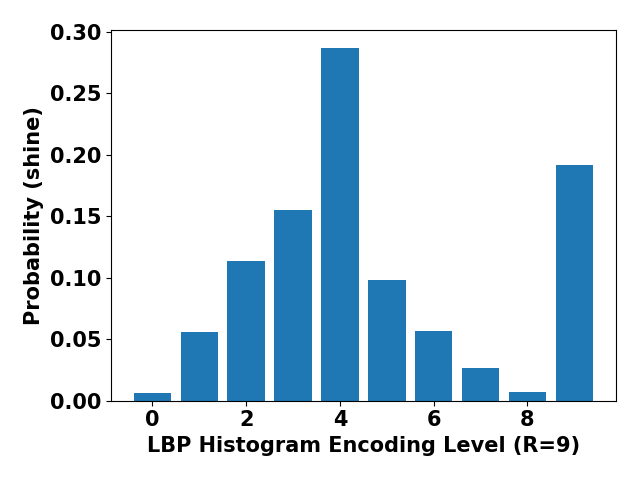
\includegraphics[width=0.245\textwidth]{../My_Code/Results/LBP_shine_R_9.png}}
    \subcaptionbox{}{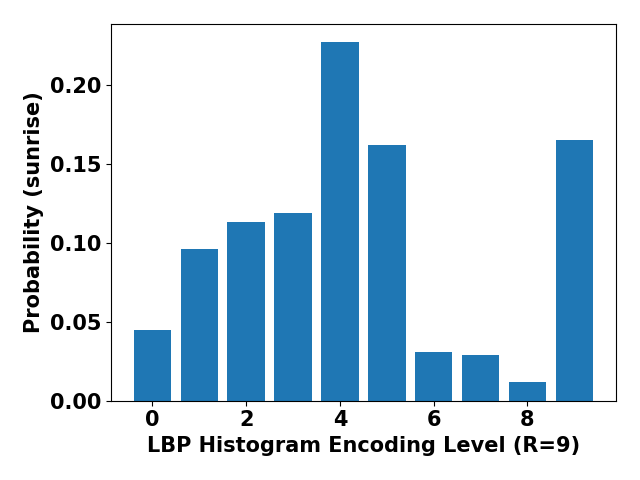
\includegraphics[width=0.245\textwidth]{../My_Code/Results/LBP_sunrise_R_9.png}}
    \caption{LBP Histograms for different local circular pattern radius (R). Each row correspond to a specific R (r=1,3,5,7,9, respectively, from top to bottom). Each column correspond to the first image of the training set in specific class.}
    \label{fig:LBP_features}
\end{figure}


\newpage
\subsection{Mean LBP Feature Vectors}
\begin{figure}[!htbp]
     \centering
     \captionsetup[subfigure]{labelformat=empty}
    \subcaptionbox{}{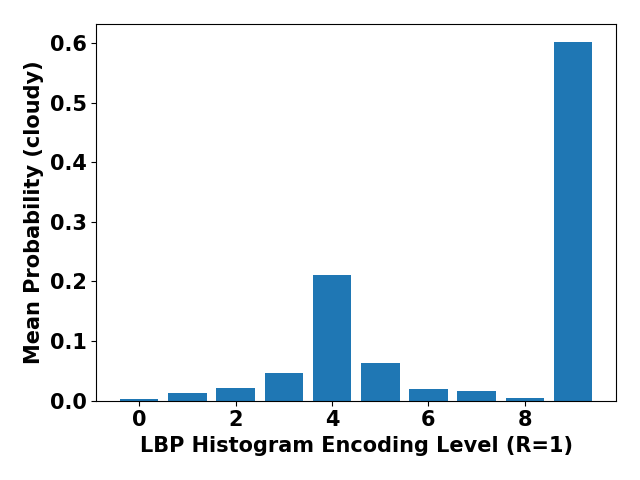
\includegraphics[width=0.245\textwidth]{../My_Code/Results/Mean_LBP_cloudy_R_1.png}}
    \subcaptionbox{}{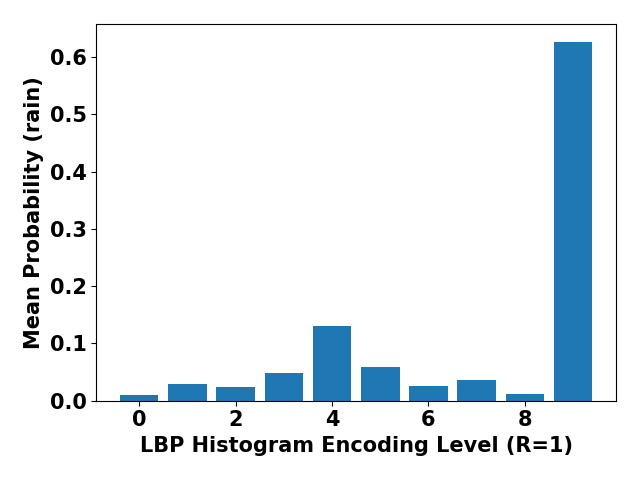
\includegraphics[width=0.245\textwidth]{../My_Code/Results/Mean_LBP_rain_R_1.png}}
    \subcaptionbox{}{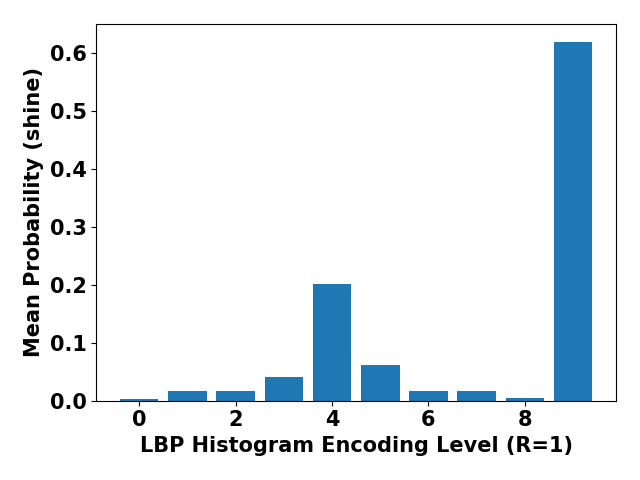
\includegraphics[width=0.245\textwidth]{../My_Code/Results/Mean_LBP_shine_R_1.png}}
    \subcaptionbox{}{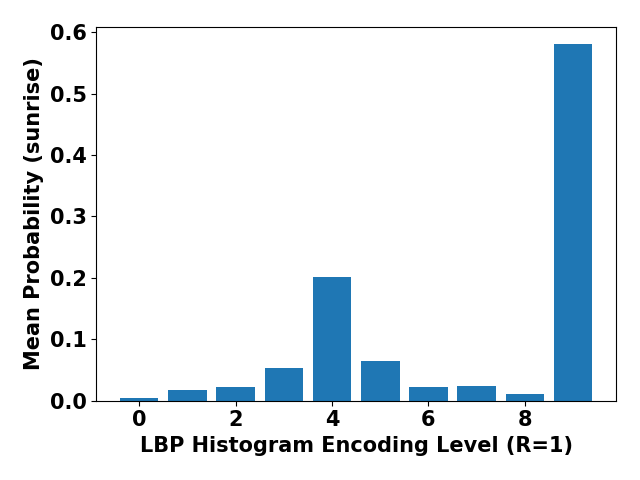
\includegraphics[width=0.245\textwidth]{../My_Code/Results/Mean_LBP_sunrise_R_1.png}}
    \subcaptionbox{}{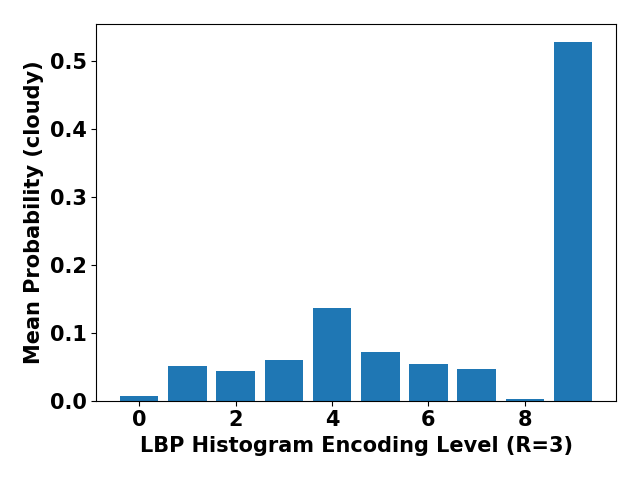
\includegraphics[width=0.245\textwidth]{../My_Code/Results/Mean_LBP_cloudy_R_3.png}}
    \subcaptionbox{}{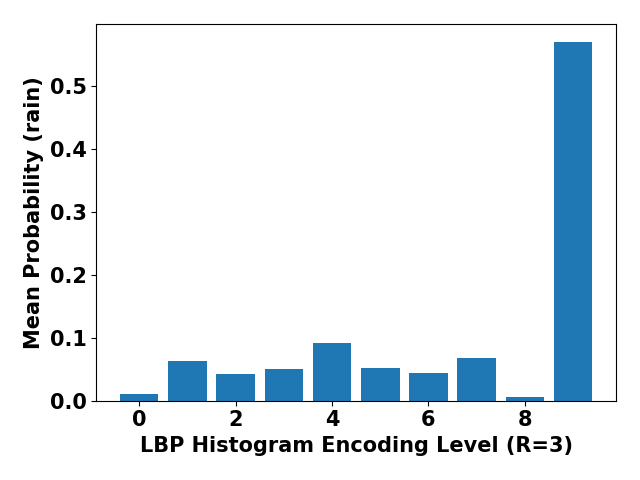
\includegraphics[width=0.245\textwidth]{../My_Code/Results/Mean_LBP_rain_R_3.png}}
    \subcaptionbox{}{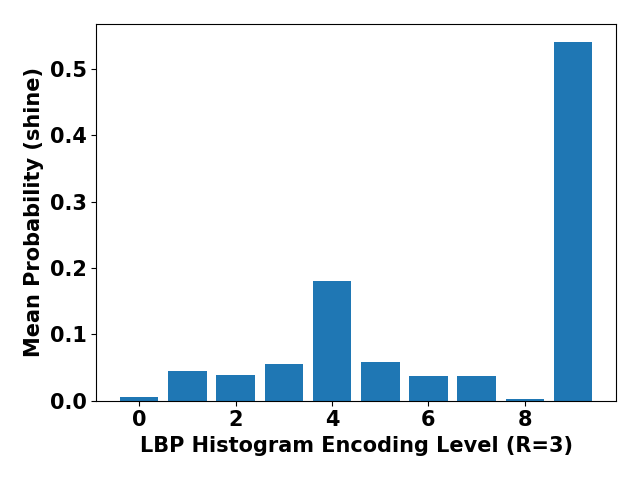
\includegraphics[width=0.245\textwidth]{../My_Code/Results/Mean_LBP_shine_R_3.png}}
    \subcaptionbox{}{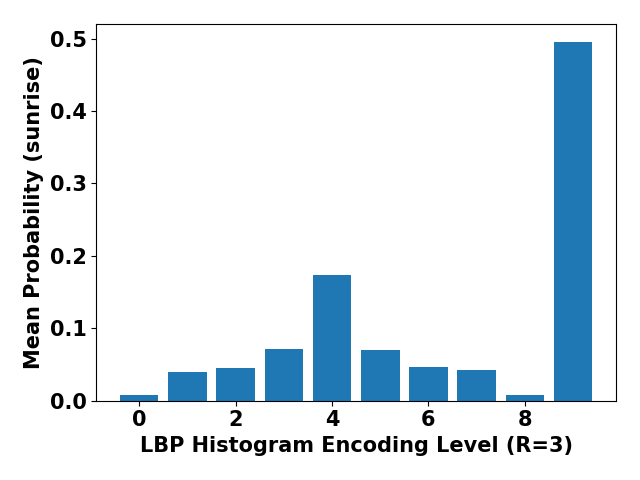
\includegraphics[width=0.245\textwidth]{../My_Code/Results/Mean_LBP_sunrise_R_3.png}}
    \subcaptionbox{}{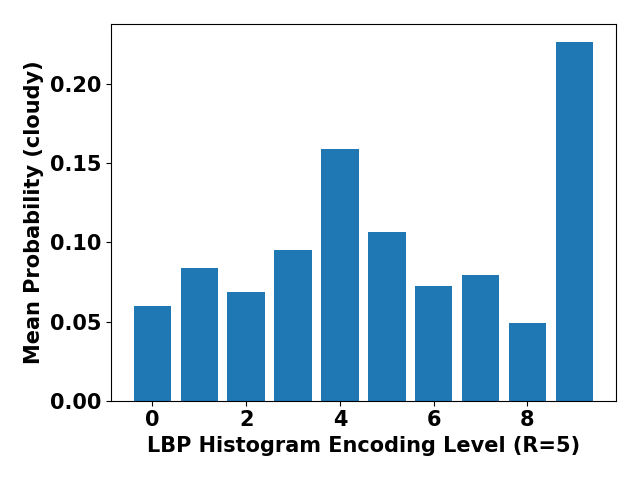
\includegraphics[width=0.245\textwidth]{../My_Code/Results/Mean_LBP_cloudy_R_5.png}}
    \subcaptionbox{}{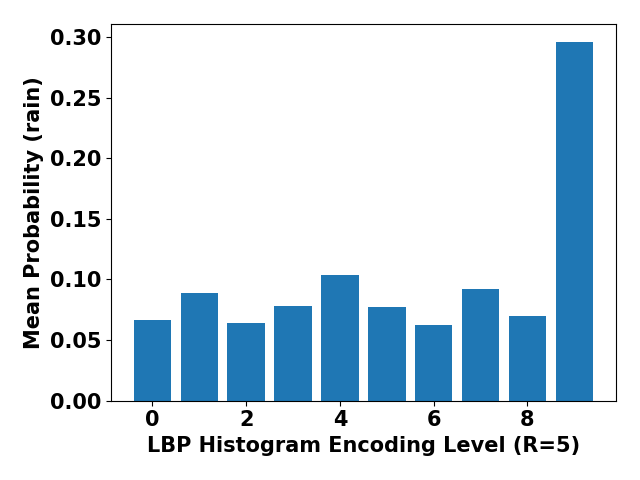
\includegraphics[width=0.245\textwidth]{../My_Code/Results/Mean_LBP_rain_R_5.png}}
    \subcaptionbox{}{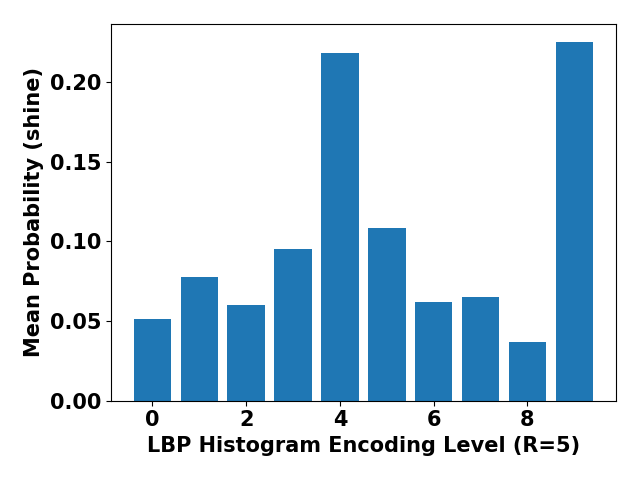
\includegraphics[width=0.245\textwidth]{../My_Code/Results/Mean_LBP_shine_R_5.png}}
    \subcaptionbox{}{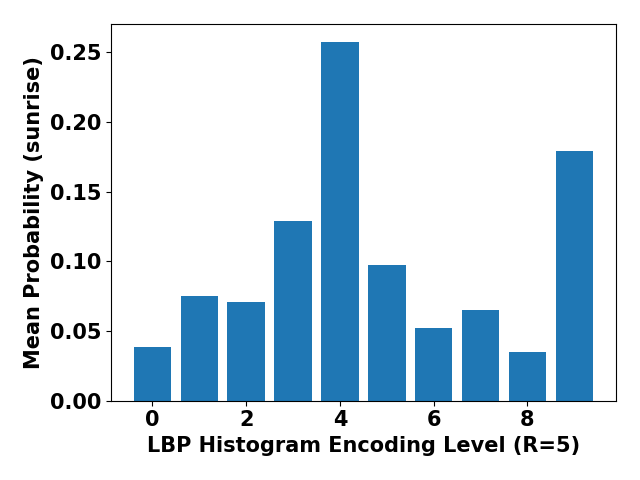
\includegraphics[width=0.245\textwidth]{../My_Code/Results/Mean_LBP_sunrise_R_5.png}}
    \subcaptionbox{}{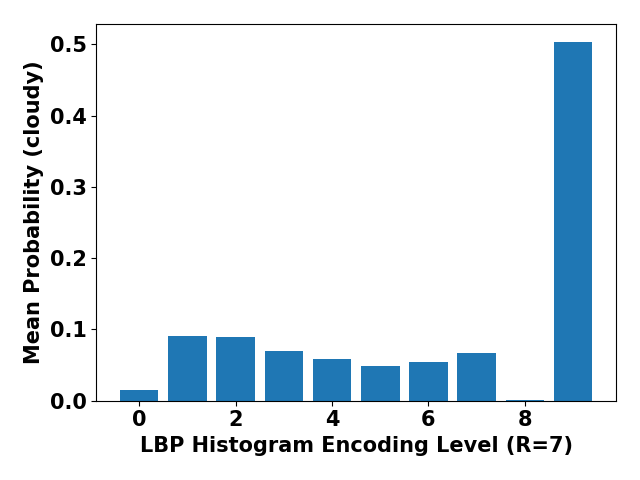
\includegraphics[width=0.245\textwidth]{../My_Code/Results/Mean_LBP_cloudy_R_7.png}}
    \subcaptionbox{}{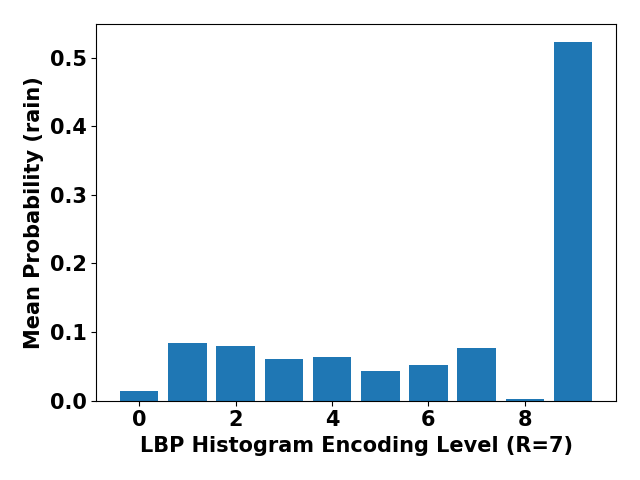
\includegraphics[width=0.245\textwidth]{../My_Code/Results/Mean_LBP_rain_R_7.png}}
    \subcaptionbox{}{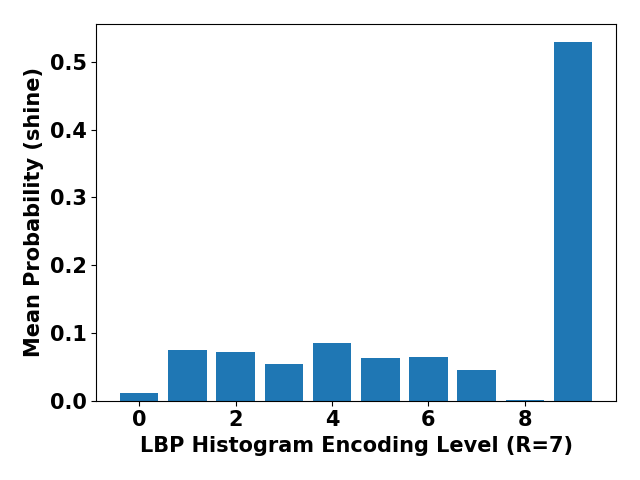
\includegraphics[width=0.245\textwidth]{../My_Code/Results/Mean_LBP_shine_R_7.png}}
    \subcaptionbox{}{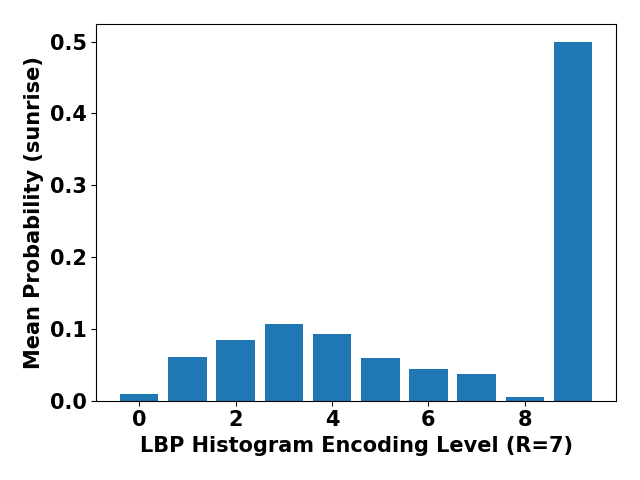
\includegraphics[width=0.245\textwidth]{../My_Code/Results/Mean_LBP_sunrise_R_7.png}}
    \subcaptionbox{}{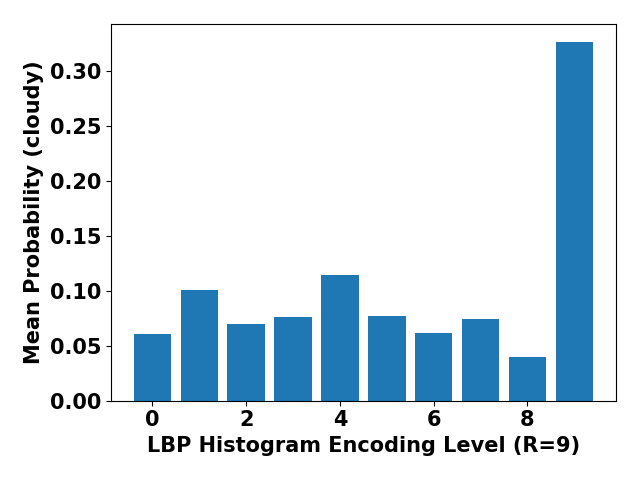
\includegraphics[width=0.245\textwidth]{../My_Code/Results/Mean_LBP_cloudy_R_9.png}}
    \subcaptionbox{}{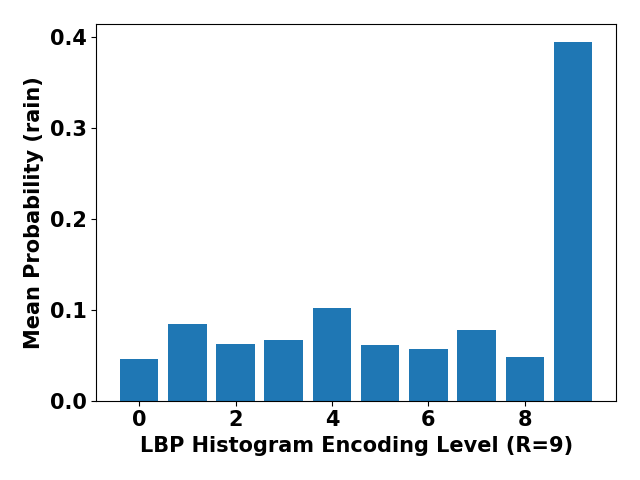
\includegraphics[width=0.245\textwidth]{../My_Code/Results/Mean_LBP_rain_R_9.png}}
    \subcaptionbox{}{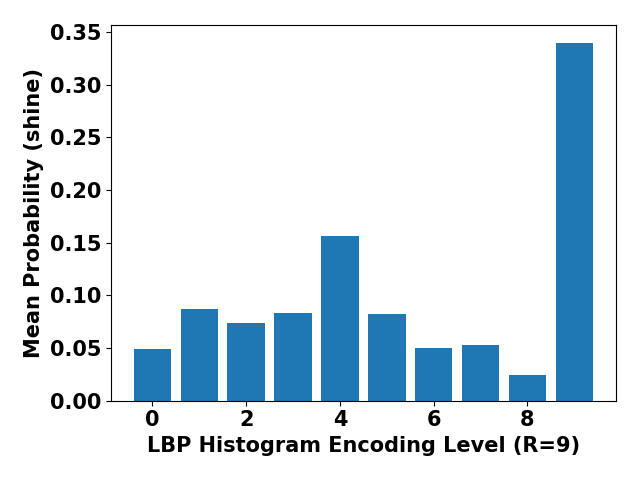
\includegraphics[width=0.245\textwidth]{../My_Code/Results/Mean_LBP_shine_R_9.png}}
    \subcaptionbox{}{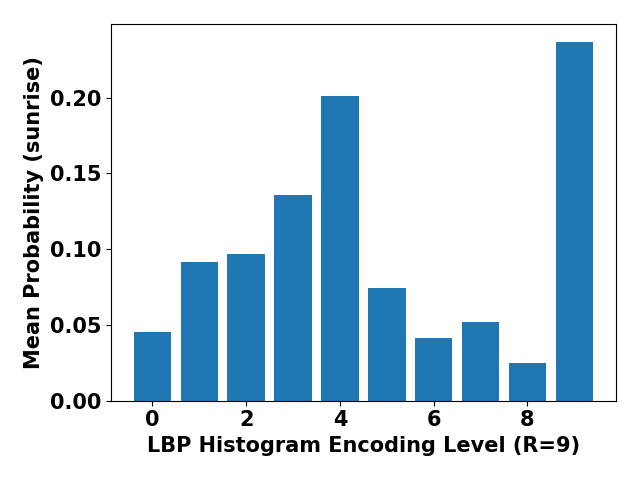
\includegraphics[width=0.245\textwidth]{../My_Code/Results/Mean_LBP_sunrise_R_9.png}}
    \caption{LBP Histograms for different local circular pattern radius (R). Each row correspond to a specific R (r=1,3,5,7,9, respectively, from top to bottom). Each column correspond to a specific class in the database. The histograms are averaged across all images within a particular class.}
    \label{fig:Mean_LBP_features}
\end{figure}

\newpage
\subsection{Accuracy of LBP Feature Extractor}
\begin{figure}[!htbp]
     \centering
     \captionsetup[subfigure]{labelformat=empty}
    \subcaptionbox{a}{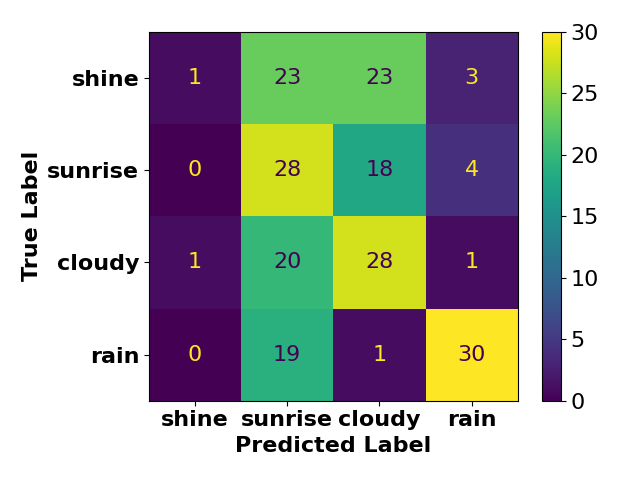
\includegraphics[width=0.328\textwidth]{../My_Code/Results/Confusion_Matrix_LBP_R_1.png}}
    \subcaptionbox{b}{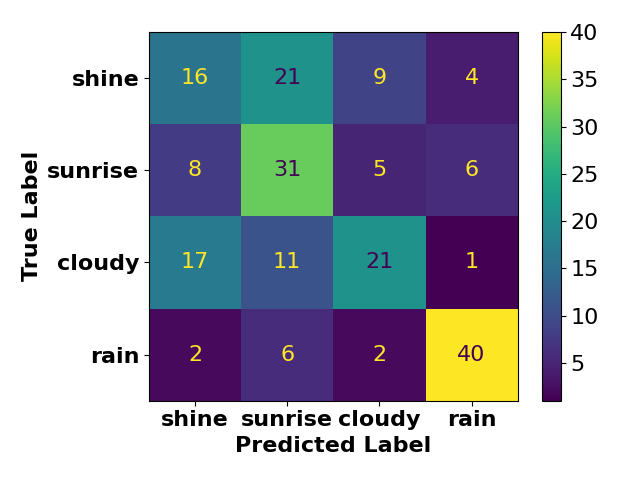
\includegraphics[width=0.328\textwidth]{../My_Code/Results/Confusion_Matrix_LBP_R_2.png}}
    \subcaptionbox{c}{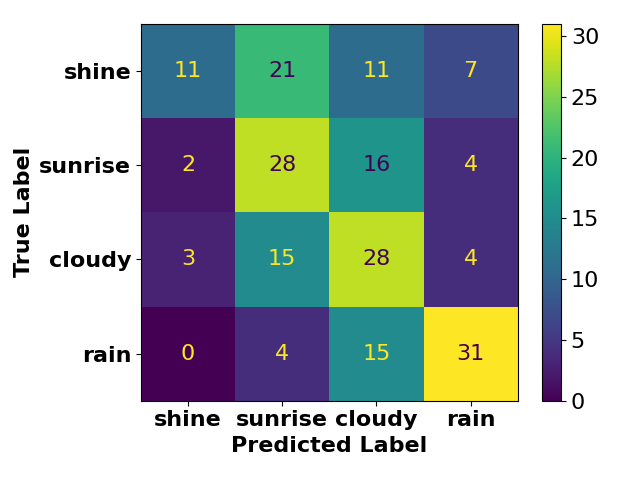
\includegraphics[width=0.328\textwidth]{../My_Code/Results/Confusion_Matrix_LBP_R_3.png}}
    \subcaptionbox{d}{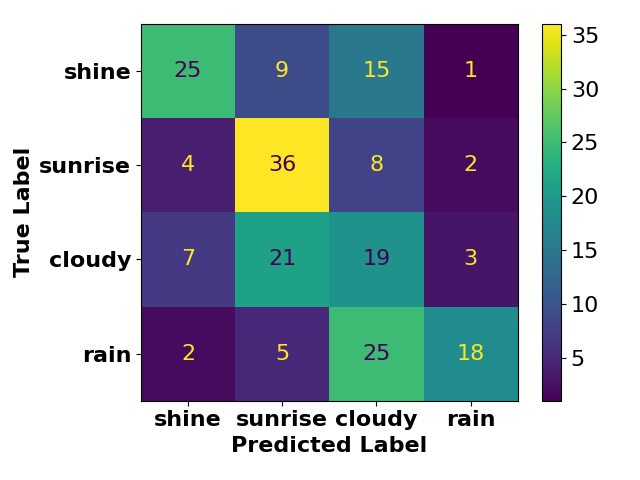
\includegraphics[width=0.328\textwidth]{../My_Code/Results/Confusion_Matrix_LBP_R_4.png}}
    \subcaptionbox{e}{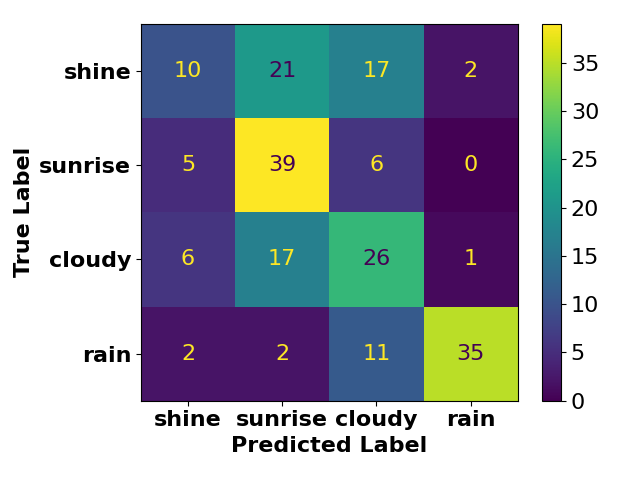
\includegraphics[width=0.328\textwidth]{../My_Code/Results/Confusion_Matrix_LBP_R_5.png}}
    \subcaptionbox{f}{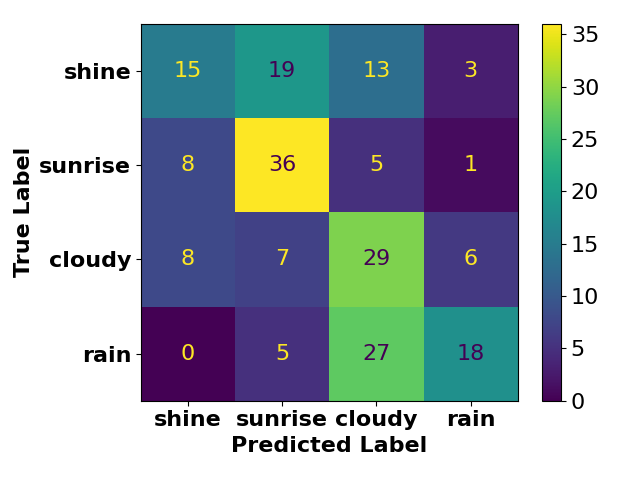
\includegraphics[width=0.328\textwidth]{../My_Code/Results/Confusion_Matrix_LBP_R_6.png}}
    \subcaptionbox{g}{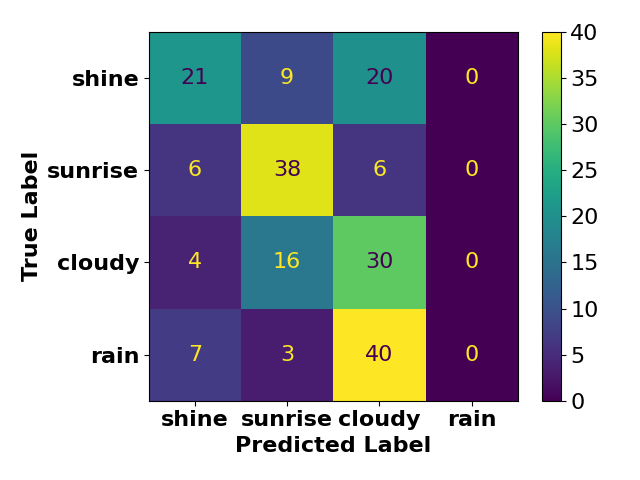
\includegraphics[width=0.328\textwidth]{../My_Code/Results/Confusion_Matrix_LBP_R_7.png}}
    \subcaptionbox{h}{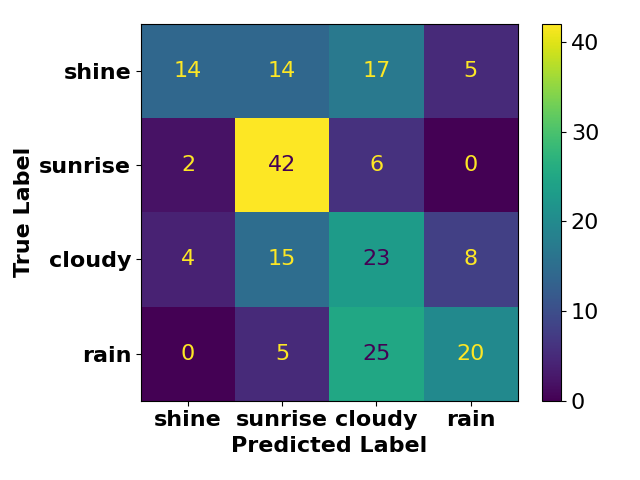
\includegraphics[width=0.328\textwidth]{../My_Code/Results/Confusion_Matrix_LBP_R_8.png}}
    \subcaptionbox{i}{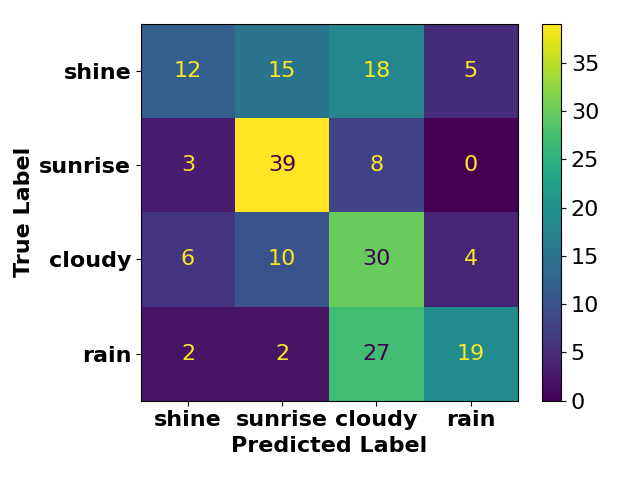
\includegraphics[width=0.328\textwidth]{../My_Code/Results/Confusion_Matrix_LBP_R_9.png}}
    \subcaptionbox{j}{\includegraphics[width=0.328\textwidth]{../My_Code/Results/Confusion_Matrix_LBP_R_10.png}}
    \subcaptionbox{k}{\includegraphics[width=0.45\textwidth]{../My_Code/Results/LBP_Accuraccy.png}}
    \caption{Confusion matrices showing class-based accuracies for different local circular pattern radius (R) in LBP. $R=1,2\cdots 9$ from (a),(b)$\cdots$ (j), respectively. (k) Accuracy of LBP method for different R.}
    \label{fig:LBP_Accuracy}
\end{figure}

\newpage
\subsection{Gram Matrices (GM)}
\begin{figure}[!htbp]
     \centering
     \captionsetup[subfigure]{labelformat=empty}
    \subcaptionbox{}{\includegraphics[width=0.245\textwidth]{../My_Code/Results/GM_Matrices/GM_cloudy1.png}}
    \subcaptionbox{}{\includegraphics[width=0.245\textwidth]{../My_Code/Results/GM_Matrices/GM_rain1.png}}
    \subcaptionbox{}{\includegraphics[width=0.245\textwidth]{../My_Code/Results/GM_Matrices/GM_shine114.png}}
    \subcaptionbox{}{\includegraphics[width=0.245\textwidth]{../My_Code/Results/GM_Matrices/GM_sunrise17.png}}
    \subcaptionbox{}{\includegraphics[width=0.245\textwidth]{../My_Code/Results/GM_Matrices/GM_cloudy10.png}}
    \subcaptionbox{}{\includegraphics[width=0.245\textwidth]{../My_Code/Results/GM_Matrices/GM_rain10.png}}
    \subcaptionbox{}{\includegraphics[width=0.245\textwidth]{../My_Code/Results/GM_Matrices/GM_shine101.png}}
    \subcaptionbox{}{\includegraphics[width=0.245\textwidth]{../My_Code/Results/GM_Matrices/GM_sunrise18.png}}
    \subcaptionbox{}{\includegraphics[width=0.245\textwidth]{../My_Code/Results/GM_Matrices/GM_cloudy100.png}}
    \subcaptionbox{}{\includegraphics[width=0.245\textwidth]{../My_Code/Results/GM_Matrices/GM_rain100.png}}
    \subcaptionbox{}{\includegraphics[width=0.245\textwidth]{../My_Code/Results/GM_Matrices/GM_shine11.png}}
    \subcaptionbox{}{\includegraphics[width=0.245\textwidth]{../My_Code/Results/GM_Matrices/GM_sunrise163.png}}
    \subcaptionbox{}{\includegraphics[width=0.245\textwidth]{../My_Code/Results/GM_Matrices/GM_cloudy108.png}}
    \subcaptionbox{}{\includegraphics[width=0.245\textwidth]{../My_Code/Results/GM_Matrices/GM_rain108.png}}
    \subcaptionbox{}{\includegraphics[width=0.245\textwidth]{../My_Code/Results/GM_Matrices/GM_shine103.png}}
    \subcaptionbox{}{\includegraphics[width=0.245\textwidth]{../My_Code/Results/GM_Matrices/GM_sunrise164.png}}
    \subcaptionbox{}{\includegraphics[width=0.245\textwidth]{../My_Code/Results/GM_Matrices/GM_cloudy112.png}}
    \subcaptionbox{}{\includegraphics[width=0.245\textwidth]{../My_Code/Results/GM_Matrices/GM_rain112.png}}
    \subcaptionbox{}{\includegraphics[width=0.245\textwidth]{../My_Code/Results/GM_Matrices/GM_shine112.png}}
    \subcaptionbox{}{\includegraphics[width=0.245\textwidth]{../My_Code/Results/GM_Matrices/GM_sunrise165.png}}
    \caption{Sample Gram matrices for different classes in the dataset. First column correspond to class 'cloudy', second column correspond to class 'rain', third column correspond to class 'shine' and the fourth column correspond to class 'sunrise'. These normalized Gram matrices are on a log scale.}
    \label{fig:GM_vectors}
\end{figure}

\newpage
\subsection{Accuracy of GM Feature Extractors}
\begin{figure}[!htbp]
     \centering
     \captionsetup[subfigure]{labelformat=empty}
    \subcaptionbox{(a)}{\includegraphics[width=0.495\textwidth]{../My_Code/Results/Confusion_Matrix_GM.png}}
    \subcaptionbox{(b)}{\includegraphics[width=0.495\textwidth]{../My_Code/Results/GM_Accuraccy.png}}
\caption{Accuracy of GM feature extractors. (a) Confusion matrix with length of GM feature vector of 1024. (b) Accuracy Improvement with respect to GM feature vector length.}
    \label{fig:GM_Results}
\end{figure}


\section{Extra Credits}
\subsection{Accuracy of Adaptve Instance Normalization (AdaIN) Feature Extractors}
\begin{figure}[!htbp]
     \centering
     \captionsetup[subfigure]{labelformat=empty}
    \subcaptionbox{(a)}{\includegraphics[width=0.495\textwidth]{../My_Code/Results/Confusion_Matrix_AdaIN.png}}
    \subcaptionbox{(b)}{\includegraphics[width=0.495\textwidth]{../My_Code/Results/AdaIN_Accuraccy.png}}
\caption{Accuracy of AdaIN feature extractors. (a) Confusion matrix with length of AdaIN feature vector of 1024. (b) Accuracy Improvement with respect to AdaIN feature vector length.}
    \label{fig:AdaIN_Results}
\end{figure}

\newpage
\section{Discussion}
\begin{itemize}
\item The LBP histogram-based feature extractor provides a maximum accuracy of $55\%$ when R=5 and P=8. LBP histogram based features are not so different for different image classes. Therefore, getting a high accuracy is extremely difficult. Also, overfitting is very common for such data.
\item The Gram matrix (GM) based feature extractor provides a maximum accuracy of $97.5\%$ when we consider the whole $512\times 512$ GM matrix as a feature vector without subsampling. However, we can achieve an accuracy over $90\%$ for a feature vector of length within 2048. The GM vector space is very high dimensional $(512\times 512)$. If we subsample it very sparsely, the accuracy will degrade, that is evident in Fig. \ref{fig:GM_Results}.
\item The Adaptive Instance Normalization (AdaIN) based feature extractor achieves a maximum accuracy of $96\%$ when we consider all of $1024$ statistical features from the output of VGG19 model. Since, the AdaIN feature vector space is not so high dimensional as of GM, we can consider all the features to gain high accuracy.
\end{itemize}

\section{Reference}
\begin{itemize}
\item Kak, A. C. (2016). Measuring texture and color in images. URL: https://engineering. purdue. edu/kak/Tutorials/TextureAndColor. pdf.
\item Kak, A. (2018). BitVector. py. Retrieved October, 28, 2018.
\item Leon A Gatys, Alexander S Ecker, and Matthias Bethge. Image style
transfer using convolutional neural networks. In Proceedings of the IEEE
conference on computer vision and pattern recognition, pages 2414–2423,
2016.
\item Gbeminiyi Ajayi. Multi-class Weather Dataset for Image Classification.
URL http://dx.doi.org/10.17632/4drtyfjtfy.1.
\item Xun Huang and Serge Belongie. Arbitrary style transfer in real-time
with adaptive instance normalization. In Proceedings of the IEEE inter-
national conference on computer vision, pages 1501–1510, 2017.
\item Tero Karras, Samuli Laine, and Timo Aila. A style-based generator
architecture for generative adversarial networks. In Proceedings of the
IEEE/CVF conference on computer vision and pattern recognition, pages
4401–4410, 2019.
\end{itemize}
\newpage
\section{Source Code}
\begin{lstlisting}[language=Python]
import os,math
import numpy as np
import cv2
import BitVector

def lbp(im,R=1,P=8,eps=0.000001,verbose=False):
	#calculates the local binary pattern of an image
	#im : input image
	#R : radius of the circular pattern
	#P : number of points to sample on the circle
	if len(im.shape)>2:
		#convert the image to grayscale
		im = cv2.cvtColor(im, cv2.COLOR_BGR2GRAY)
	image_width = im.shape[1]
	image_height = im.shape[0]
	LBP_HIST = {kx:0 for kx in range(P+2)}

	for ix in range(R,image_height-R):
		for jx in range(R,image_width-R):
			#for each of these pixels generate a binary pattern
			PATTERN = list()
			for p in range(0,P):
				NEIGHBOUR_POINTS_ON_CIRCLE = np.array([R*np.cos(2*np.pi*p/P),R*np.sin(2*np.pi*p/P)])
				NEIGHBOUR_POINTS_ON_CIRCLE[abs(NEIGHBOUR_POINTS_ON_CIRCLE)<eps] = 0

				kx,lx = ix+NEIGHBOUR_POINTS_ON_CIRCLE[0],jx+NEIGHBOUR_POINTS_ON_CIRCLE[1]
				kxb,lxb = math.floor(kx),math.floor(lx)
				del_kx,del_lx = kx-kxb,lx-lxb
				if del_kx < eps and del_lx<eps:
					IMAGE_AT_P = im[kxb,lxb]
				elif del_lx < eps:
					IMAGE_AT_P = (1-del_kx)*im[kxb,lxb] + del_kx*im[kxb+1,lxb]
				elif del_kx < eps:
					IMAGE_AT_P = (1-del_lx)*im[kxb,lxb] + del_lx*im[kxb,lxb+1]
				else:
					IMAGE_AT_P = im[kxb,lxb]*(1-del_kx)*(del_lx)+im[kxb,lxb+1]*del_lx*(1-del_kx)+im[kxb+1,lxb]*del_kx*(1-del_lx)+im[kxb+1,lxb+1]*del_kx*del_lx;
				if IMAGE_AT_P>=im[ix,jx]:
					PATTERN.append(1)
				else:
					PATTERN.append(0)

			BITVECTOR = BitVector.BitVector(bitlist=PATTERN)
			CIRC_SHIFT_INTVL = [int(BITVECTOR<<1) for _ in range(P)]
			MINBV = BitVector.BitVector(intVal=min(CIRC_SHIFT_INTVL),size=P)
			BVRUNS = MINBV.runs()
			if len(BVRUNS) > 2:
				LBP_HIST[P+1] += 1
				ENCODING = P+1
			elif len(BVRUNS) == 1 and BVRUNS[0][0] == '1':
				LBP_HIST[P] += 1
				ENCODING = P
			elif len(BVRUNS) == 1 and BVRUNS[0][0] == '0':
				LBP_HIST[0] += 1
				ENCODING = 0
			else:
				LBP_HIST[len(BVRUNS[1])] += 1
				ENCODING = len(BVRUNS[1])
			if verbose:
				print('Pixel [i,j] = [',ix,',',jx,']')
				print('Pattern = ',PATTERN)
				print('minbv = ',MINBV)
				print('encoding = ',ENCODING)
				print('\n')
	if verbose:
		print('LBP Histogram = ',LBP_HIST)
	return LBP_HIST

import os
import cv2
import lbp
import random
import numpy as np
from joblib import Parallel, delayed
import vgg
from skimage import io, transform
import matplotlib.pyplot as plt
from sklearn.pipeline import make_pipeline
from sklearn.preprocessing import StandardScaler
from sklearn import svm
from sklearn.metrics import ConfusionMatrixDisplay, confusion_matrix

def prepare_LBP_histograms(ix,images,dir,LBP_SAVE_DIR,name,params):
	R,P,vb = params
	if images[ix][-4:]=='.jpg':
		save_file_name = LBP_SAVE_DIR+'/'+name+'/'+images[ix][:-4]+'.npz'
		if not os.path.exists(save_file_name):
			try:
				print(name,'---R=',R,'---',ix+1,'/',len(images),'---',images[ix])
				im = cv2.imread(dir+'/'+images[ix])
				im = cv2.resize(im,(64,64),interpolation=cv2.INTER_AREA)
				LBP_HISTOGRAM = lbp.lbp(im,R=R,P=P,verbose=vb)
				total_count=0
				for key,val in LBP_HISTOGRAM.items():
					total_count = total_count + val
				for key,val in LBP_HISTOGRAM.items():
					LBP_HISTOGRAM[key] = round(val/total_count,3)
				np.savez(save_file_name,LBP_HISTOGRAM=LBP_HISTOGRAM)
			except Exception as ex:
				print('Problem in reading file - ',images[ix],'---',ex)

def prepare_GM_features(image,model,dir,GM_SAVE_DIR,name,idx,NI):
	save_file_name = GM_SAVE_DIR+'/'+name+'/'+image[:-4]+'.npz'
	if not os.path.exists(save_file_name):
		try:
			print(name,'---',idx+1,'/',NI,'---',image)
			im = cv2.imread(dir+'/'+image)
			im = cv2.resize(im,(256,256),interpolation=cv2.INTER_AREA)
			F = model(im) #Get the feature vector
			F = np.reshape(F,[F.shape[0],F.shape[1]*F.shape[2]])
			G = np.matmul(F,F.T)#calculate the gram matrix
			G = G/np.max(G)#Normalize the gram matrix
			G = np.reshape(G,[1,np.prod(G.shape)])
			np.savez(save_file_name,GM_FEATURE_VECTOR=G)
		except Exception as ex:
			print('Problem in reading file - ',image,'---',ex)

def prepare_AdaIN_features(image,model,dir,AdaIN_SAVE_DIR,name,idx,NI):
	save_file_name = AdaIN_SAVE_DIR+'/'+name+'/'+image[:-4]+'.npz'
	if not os.path.exists(save_file_name):
		try:
			print(name,'---',idx+1,'/',NI,'---',image)
			im = cv2.imread(dir+'/'+image)
			im = cv2.resize(im,(256,256),interpolation=cv2.INTER_AREA)
			F = model(im) #Get the feature vector
			F = np.reshape(F,[F.shape[0],F.shape[1]*F.shape[2]])
			mean_per_channel = np.mean(F,axis=1)
			variance_per_channel = np.var(F,axis=1)
			AD = np.stack((mean_per_channel,variance_per_channel),axis=1)
			AD = AD/np.max(AD)
			AD = np.reshape(AD,[1,np.prod(AD.shape)]).squeeze()
			np.savez(save_file_name,AdaIN_FEATURE_VECTOR=AD)
		except Exception as ex:
			print('Problem in reading file - ',image,'---',ex)

def plot_GM(G,name,eps=1e-14):
	if not os.path.exists('./Results/GM_Matrices'):
		os.makedirs('./Results/GM_Matrices')
	G = G+eps#to avoid nans in the log scale
	G = np.log10(G)
	plt.figure()
	plt.rcParams.update({'font.size': 16})
	plt.imshow(G)
	plt.colorbar()
	plt.xticks(fontweight=600,fontsize=15)
	plt.yticks(fontweight=600,fontsize=15)
	plt.tight_layout()
	plt.savefig('./Results/GM_Matrices/'+name+'.png')

def plot_LBP(LBP_Features,LBP_Labels,classes,R):
	for ix in range(1,len(classes)+1):
		ind = np.argwhere(LBP_Labels==ix).squeeze()
		Class_LBP = LBP_Features[ind,:]
		Mean_Class_LBP = np.mean(Class_LBP,axis=0)
		plt.figure()
		plt.bar(np.arange(0,10).tolist(),Mean_Class_LBP.tolist())
		plt.xticks(fontweight=600,fontsize=15)
		plt.yticks(fontweight=600,fontsize=15)
		plt.xlabel('LBP Histogram Encoding Level (R='+str(R)+')',fontweight=800,fontsize=15)
		plt.ylabel('Mean Probability ('+classes[ix-1]+')',fontweight=800,fontsize=15)
		plt.tight_layout()
		plt.savefig('./Results/Mean_LBP_'+classes[ix-1]+'_R_'+str(R)+'.png')

		plt.figure()
		plt.bar(np.arange(0,10).tolist(),Class_LBP[1,:].tolist())
		plt.xticks(fontweight=600,fontsize=15)
		plt.yticks(fontweight=600,fontsize=15)
		plt.xlabel('LBP Histogram Encoding Level (R='+str(R)+')',fontweight=800,fontsize=15)
		plt.ylabel('Probability ('+classes[ix-1]+')',fontweight=800,fontsize=15)
		plt.tight_layout()
		plt.savefig('./Results/LBP_'+classes[ix-1]+'_R_'+str(R)+'.png')

def data_load(dir,mode,classes,params):
	D = os.listdir(dir)
	FEATURES = list()
	LABELS = list()
	COUNTS = {tx:0 for tx in range(1,len(classes)+1)}
	for ix in range(0,len(D)):
		X = np.load(dir+'/'+D[ix],allow_pickle=True)
		if mode.upper() == 'LBP':
			V = X['LBP_HISTOGRAM'].item()
			temp = np.array([V[k] for k in range(0,10)])
			temp = np.reshape(temp,[1,10])
			FEATURES.append(temp)
		elif mode.upper() == 'GM':
			G = X['GM_FEATURE_VECTOR']
			if params[0] > 0:
				G = G[0,:params[0]]
				G = np.reshape(G,[1,G.shape[0]])
			FEATURES.append(G)
		elif mode.upper() == 'ADAIN':
			A = X['AdaIN_FEATURE_VECTOR']
			A = np.reshape(A,[1,A.shape[0]])
			if params[0] > 0:
				A = A[0,:params[0]]
				A = np.reshape(A,[1,A.shape[0]])
			FEATURES.append(A)
		else:
			print('Please provide a valid moode, either LBP/GM/AdaIN')
		temp = [1 if classes[jx] in D[ix] else 0 for jx in range(0,len(classes))]
		class_id = np.argmax(temp)+1
		COUNTS[class_id] += 1
		LABELS.append(class_id)

	FEATURES = np.array(FEATURES)
	FEATURES = np.reshape(FEATURES,[FEATURES.shape[0],FEATURES.shape[2]])
	LABELS = np.array(LABELS)
	return FEATURES,LABELS,COUNTS

def train(train_dir,test_dir,mode,classes,FEATURE_VECTOR_LENGTH,verbose=False,plot_cfm=False,params=['']):
	X_train,Y_train,COUNTS = data_load(train_dir,mode,classes,[FEATURE_VECTOR_LENGTH])
	#print('AdaIN Training Features = ',X_train_AdaIN.shape)
	#print('AdaIN Training Labels = ',Y_train_AdaIN.shape)
	#print('AdaIN Training Labels Distribution = ',COUNTS)
	P = svm.SVC(decision_function_shape='ovo')
	P.fit(X_train,Y_train)
	X_test,Y_test,COUNTS = data_load(test_dir,mode,classes,[FEATURE_VECTOR_LENGTH])
	#print('AdaIN Testing Features = ',X_test_AdaIN.shape)
	#print('AdaIN Testing Labels = ',Y_test_AdaIN.shape)
	#print('AdaIN Testing Labels Distribution = ',COUNTS)
	YP_test = P.predict(X_test)
	ACCURACY = P.score(X_test,Y_test)
	if verbose:
		print(mode,' Accuracy, featurevector length = ',FEATURE_VECTOR_LENGTH,',    ',mode,' Accuracy = ',np.round(ACCURACY*100,2),'%')
	if plot_cfm:
		#plot_confusion_matrix(P,X_test,Y_test,class_names=classes)
		fig = plt.figure()
		plt.rcParams.update({'font.size': 16})
		cm = confusion_matrix(Y_test, YP_test)
		cmd = ConfusionMatrixDisplay(cm, display_labels=classes)
		P = cmd.plot()
		plt.xticks(fontweight=600,fontsize=16)
		plt.yticks(fontweight=600,fontsize=16)
		plt.xlabel('Predicted Label',fontweight=800,fontsize=16)
		plt.ylabel('True Label',fontweight=800,fontsize=16)
		plt.tight_layout()
		plt.savefig('./Results/Confusion_Matrix_'+mode+params[0]+'.png')
	return [X_train, Y_train, X_test, Y_test, ACCURACY]


def plot_accuracy(fnames,mode,xlabel=None):
	fig = plt.figure()
	M = np.load(fnames[0])
	Acc = M[mode+'_Accuracies'].tolist()
	X = M['FEATURE_VECTOR_LENGTH'].tolist()
	plt.plot(X,Acc,linewidth=2)
	#plt.xscale("log")
	ylim_min = 30
	ylim_max=101
	plt.ylim(ylim_min,ylim_max)
	plt.xticks(fontweight=600,fontsize=10)
	plt.yticks(np.arange(ylim_min, ylim_max, 5.0),fontweight=600,fontsize=10)
	xlabel = xlabel[0] if xlabel else mode+' Feature Vector Length'
	ylabel = 'Accuracy (%)'
	plt.xlabel(xlabel,fontweight=800,fontsize=12)
	plt.ylabel(ylabel,fontweight=800,fontsize=12)
	plt.grid()
	plt.tight_layout()
	plt.savefig('./Results/'+mode+'_Accuraccy.png')

def Main():
	R = 1#radius of the circular pattern
	P = 8#number of points to sample on the circle
	classes = ['shine','sunrise','cloudy','rain']
	if not os.path.exists('./Results'):
		os.makedirs('./Results')

	image_dir = '../data'
	train_dir = image_dir+'/training'
	test_dir = image_dir+'/testing'
	training_images = os.listdir(train_dir)
	testing_images = os.listdir(test_dir)
	###############################################################################################################
	##########   Test the LBP Generator
	'''
	fname = ''
	TEXTURE = 'random'
	if fname:
		im = cv2.imread(fname)
	else:
		#im = np.ceil(np.random.rand(4,4)*10).astype(int)#random
		im = np.array([[5,4,2,4,2,2,4,0],[4,2,1,2,1,0,0,2],[2,4,4,0,4,0,2,4],[4,1,5,0,4,0,5,5],[0,4,4,5,0,0,3,2],[2,0,4,3,0,3,1,2],[5,1,0,0,5,4,2,3],[1,0,0,4,5,5,0,1]])#arbitrary
		#im = np.array([[5,0,5,0,5,0,5,0],[5,0,5,0,5,0,5,0],[5,0,5,0,5,0,5,0],[5,0,5,0,5,0,5,0],[5,0,5,0,5,0,5,0],[5,0,5,0,5,0,5,0],[5,0,5,0,5,0,5,0],[5,0,5,0,5,0,5,0]])#vertical
		#im = np.array([[5,5,5,5,5,5,5,5],[0,0,0,0,0,0,0,0],[5,5,5,5,5,5,5,5],[0,0,0,0,0,0,0,0],[5,5,5,5,5,5,5,5],[0,0,0,0,0,0,0,0],[5,5,5,5,5,5,5,5],[0,0,0,0,0,0,0,0]])#horizontal
		#im = np.array([[0,5,0,5,0,5,0,5],[5,0,5,0,5,0,5,0],[0,5,0,5,0,5,0,5],[5,0,5,0,5,0,5,0],[0,5,0,5,0,5,0,5],[5,0,5,0,5,0,5,0],[0,5,0,5,0,5,0,5],[5,0,5,0,5,0,5,0]])#checkerboard

	if len(im.shape)>2:
		#convert the image to grayscale
		im = cv2.cvtColor(im, cv2.COLOR_BGR2GRAY)

	print('image = \n',im)
	LBP_HISTOGRAM = lbp.lbp(im,R=R,P=P,verbose=1)
	'''

	###############################################################################################################
	##########	 Generate LBP features for all images
	for R in range(1,11):
		LBP_SAVE_DIR = image_dir+'/LBP_HISTOGRAMS/R_'+str(R)
		if not os.path.exists(LBP_SAVE_DIR):
			os.makedirs(LBP_SAVE_DIR)
			os.makedirs(LBP_SAVE_DIR+'/training')
			os.makedirs(LBP_SAVE_DIR+'/testing')
		parameters = [R,P,0]
		Parallel(n_jobs=16)(delayed(prepare_LBP_histograms)(ix,training_images,train_dir,LBP_SAVE_DIR,'training',parameters) for ix in range(len(training_images)))
		Parallel(n_jobs=16)(delayed(prepare_LBP_histograms)(ix,testing_images,test_dir,LBP_SAVE_DIR,'testing',parameters) for ix in range(len(testing_images)))

	###############################################################################################################
	##########	 Generate GM features for all images
	#Prepare Gram-matrix Features from VGG Network
	# Load the model and the provided pretrained weights
	GM_SAVE_DIR = image_dir+'/GM_FEATURES'
	if not os.path.exists(GM_SAVE_DIR):
		os.makedirs(GM_SAVE_DIR)
		os.makedirs(GM_SAVE_DIR+'/training')
		os.makedirs(GM_SAVE_DIR+'/testing')
	VGG19_Model = vgg.VGG19()
	VGG19_Model.load_weights('vgg_normalized.pth')
	NI = len(training_images)
	for ix in range(0,NI):
		if training_images[ix][-4:] in ['.jpg','.JPG','.png','.PNG']:
			prepare_GM_features(training_images[ix],VGG19_Model,train_dir,GM_SAVE_DIR,'training',ix,NI)
	NI = len(testing_images)
	for ix in range(0,NI):
		if testing_images[ix][-4:] in ['.jpg','.JPG','.png','.PNG']:
			prepare_GM_features(testing_images[ix],VGG19_Model,test_dir,GM_SAVE_DIR,'testing',ix,NI)

	###############################################################################################################
	##########	 Generate AdaIN features for all images
	#Prepare AdaIN features from VGG Network
	# Load the model and the provided pretrained weights
	AdaIN_SAVE_DIR = image_dir+'/AdaIN_FEATURES'
	if not os.path.exists(AdaIN_SAVE_DIR):
		os.makedirs(AdaIN_SAVE_DIR)
		os.makedirs(AdaIN_SAVE_DIR+'/training')
		os.makedirs(AdaIN_SAVE_DIR+'/testing')
	VGG19_Model = vgg.VGG19()
	VGG19_Model.load_weights('vgg_normalized.pth')
	NI = len(training_images)
	for ix in range(0,NI):
		if training_images[ix][-4:] in ['.jpg','.JPG','.png','.PNG']:
			prepare_AdaIN_features(training_images[ix],VGG19_Model,train_dir,AdaIN_SAVE_DIR,'training',ix,NI)
	NI = len(testing_images)
	for ix in range(0,NI):
		if testing_images[ix][-4:] in ['.jpg','.JPG','.png','.PNG']:
			prepare_AdaIN_features(testing_images[ix],VGG19_Model,test_dir,AdaIN_SAVE_DIR,'testing',ix,NI)



	###############################################################################################################
	##########	 Plot the GM Feature matrix for a single image
	for image_id in range(1,100):
		try:
			X = np.load('../data/GM_FEATURES/training/'+training_images[image_id][:-4]+'.npz',allow_pickle=True)
			G = X['GM_FEATURE_VECTOR']
			G = np.reshape(G,[512,512])
			plot_GM(G,'GM_'+training_images[image_id][:-4])
		except:
			continue

	###############################################################################################################
	##########	 Training with GM Features
	if not os.path.exists('./Results/GM_Accuracies.npz'):
		GM_Accuracies = list()
		FEATURE_VECTOR_LENGTH = np.arange(1,512,2).tolist()
		FEATURE_VECTOR_LENGTH += np.arange(512,100000+512,1024).tolist()
		for kx in range(0,len(FEATURE_VECTOR_LENGTH)):
			#kx = FEATURE_VECTOR_LENGTH
			plot_cfm = True if FEATURE_VECTOR_LENGTH[kx]==100000 else False
			[_,_,_,_,GM_ACCURACY] = train('../data/GM_FEATURES/training','../data/GM_FEATURES/testing','GM',classes,FEATURE_VECTOR_LENGTH[kx],verbose=1,plot_cfm=plot_cfm)
			GM_Accuracies.append(np.round(GM_ACCURACY*100,2))
		np.savez('./Results/GM_Accuracies.npz',GM_Accuracies=GM_Accuracies,FEATURE_VECTOR_LENGTH=FEATURE_VECTOR_LENGTH)
	plot_accuracy(['./Results/GM_Accuracies.npz'],'GM')


	###############################################################################################################
	##########	 Training with LBP Features
	LBP_Accuracies = list()
	for R in range(1,11):
		[X_train_LBP,Y_train_LBP,_,_,LBP_ACCURACY] = train('../data/LBP_HISTOGRAMS/R_'+str(R)+'/training','../data/LBP_HISTOGRAMS/R_'+str(R)+'/testing','LBP',classes,-1,verbose=1,plot_cfm=True,params=['_R_'+str(R)])
		LBP_Accuracies.append(np.round(LBP_ACCURACY*100,2))
		plot_LBP(X_train_LBP,Y_train_LBP,classes,R)
	np.savez('./Results/LBP_Accuracies.npz',LBP_Accuracies=LBP_Accuracies,FEATURE_VECTOR_LENGTH=[s for s in range(1,11)])
	plot_accuracy(['./Results/LBP_Accuracies.npz'],'LBP',xlabel=['LBP Radius of circular patter, R (#pixels)'])


	###############################################################################################################
	##########	 Training with AdaIN Features
	if not os.path.exists('./Results/AdaIN_Accuracies.npz'):
		AdaIN_Accuracies = list()
		FEATURE_VECTOR_LENGTH = np.arange(1,512*2+5,5).tolist()
		for kx in range(0,len(FEATURE_VECTOR_LENGTH)):
			#kx = FEATURE_VECTOR_LENGTH
			plot_cfm = True if FEATURE_VECTOR_LENGTH[kx]==1024 else False
			[_,_,_,_,AdaIN_ACCURACY] = train('../data/AdaIN_FEATURES/training','../data/AdaIN_FEATURES/testing','AdaIN',classes,FEATURE_VECTOR_LENGTH[kx],verbose=1,plot_cfm=plot_cfm)
			AdaIN_Accuracies.append(np.round(AdaIN_ACCURACY*100,2))
		np.savez('./Results/AdaIN_Accuracies.npz',AdaIN_Accuracies=AdaIN_Accuracies,FEATURE_VECTOR_LENGTH=FEATURE_VECTOR_LENGTH)

	plot_accuracy(['./Results/AdaIN_Accuracies.npz'],'AdaIN')


Main()

\end{lstlisting}
\end{document}

